\section{Diagramme des cas d'utilisation}

Nous avons réalisé un schéma des cas d'utilisations, visible en figure \vref{usecase} afin de synthétiser les besoins de l'utilisateur, pour offrir une vision simplifiée du système. Nous rappellerons brièvement les fonctionnalités par la suite.

\begin{figure}[h]
\begin{center}
    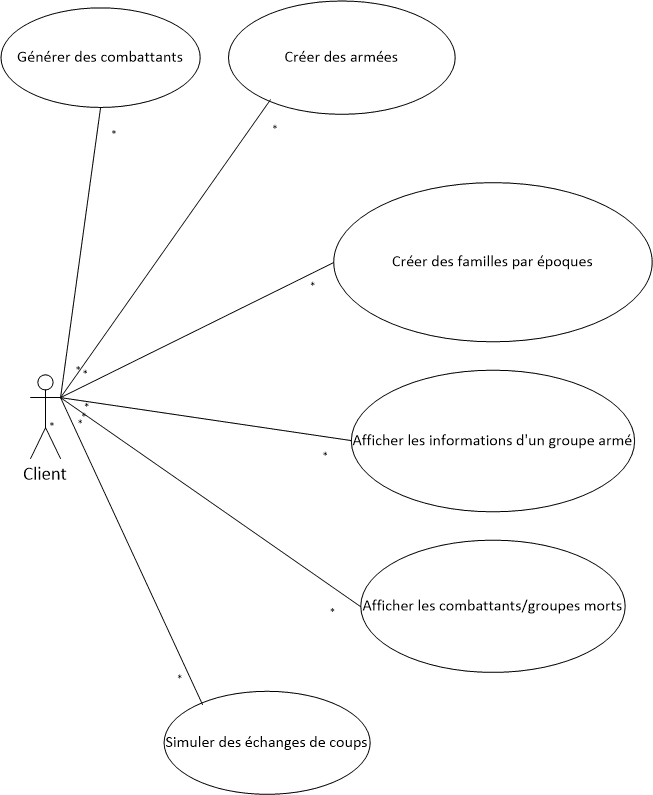
\includegraphics[width=12cm]{diagramme-usecase}
\end{center}
    \caption{Diagramme de cas d'utilisation}
    \label{usecase}                      
\end{figure}

\subsubsection{Générer des combattants}

Le client peut générer un combattant d'une classe spécifique. Il génère un combattant en utilisant un des types disponibles. Il doit spécifier l'armement du combattant après l'avoir généré.

\subsubsection{Simuler des échanges de coups}

Si des combattants ont été auparavant générés, ils peuvent s'échanger des coups, qu'ils soient équipés ou non.
Un combattant pourra frapper une cible ou parer un coups.

\subsubsection{Créer des armées}

Les armées sont composées d'éléments qui peuvent être des groupes de combattants ou des combattants. Les armées
peuvent frapper une cible ou parer une attaque.

\subsubsection{Afficher les informations d'un groupe armé}

Le client peut afficher les combattants d'un groupe armé ou compter les effectifs d'un groupe armé.

\subsubsection{Afficher les combattants morts et les groupes décimés}

Le client peut être averti du décès d'un combattant ou de l'éradication d'un groupe armé. Il peut prévenir les
amis d'un combattant du décès de celui-ci. Il peut aussi être averti du nombre de morts au fur et à mesure de
l'évolution des combats.

\subsubsection{Créer des familles de combattants par époques historiques}

Le client peut créer des combattants spécifiques à une époque et les équiper avec le type d'armement conforme
à cette époque. Par exemple, un guerrier Cromagnon ne se verra pas équipé d'une armure Terminator.